% !TEX root = main.tex

\subsection{Evaluation set-up}
\label{ssec:set_up}

We probe the ability of the proposed GP-TS to,
given a dataset, a TLM architecture, and a computational budget,
efficiently pre-train well-performing language models.
We scrutinize pre-training performance of a specific TLM architecture under equal experimental conditions 
and do not compare performance to state-of-the-art, large-scale TLMs.

For our experiments,
we incorporate RoBERTa~\citep{roberta} as implemented by~\citet{fairseq}
%as a module in our framework
in our Python implementation of GP-TS\footnote{
	Code available at~\href{https://github.com/iurteaga/gp_ts_nlp}{https://github.com/iurteaga/gp\_ts\_nlp}.
} as in Algorithm~\ref{alg:ts_pretrain_hyperparams}
---Appendix~\ref{asec:implementation_details_gp} provides implementation and configuration details.
%with GP modules in GPyTorch~\citep{gpytorch}
%---implementation and configuration details are provided in Appendix~\ref{asec:implementation_details_gp}.
%We fix the seed for the execution of RoBERTa pre-training and fine-tuning,
%but run five different realizations of the proposed GP-TS:
%\ie we quantify the performance variability induced by the stochastic bandit decisions.
We compare pre-training performance of RoBERTa models
based on a grid-search over masking hyperparameters ---as executed by~\citet{roberta}---
to RoBERTa models pre-trained by GP-TS\footnote{
	We do not execute any other hyperparameter optimization.
}.
%
We focus our evaluation on MLM validation loss and downstream per-task accuracy metrics,
and report the negligible computational overhead of pre-training with GP-TS in Appendix~\ref{asec:computational_overhead}. 

We study two variants of GP-TS, depending on the masking hyperparameters it optimizes:
\begin{enumerate}
	\vspace*{-1ex}
	\item \texttt{GP-TS $\rho$}, where the bandit arm is the masking probability $\rho$ of replacing an input token with the \textit{mask} token
	(other hyperparameters are fixed to default $\gamma=0.1$ and $\lambda=0.1$ values as in~\citet{roberta});
	and 
	\vspace*{-1ex}
	\item \texttt{GP-TS $\psi=\left(\rho, \gamma, \lambda\right)$},
	where GP-TS optimizes over all MLM dynamic masking hyperparameters:
	the bandit search space is a three-dimensional hypercube $\Psi$
	with no expert guidance. %on hyperparameter selection.
	\vspace*{-1ex}
\end{enumerate}

%\vspace*{-1ex}
\paragraph*{Pre-training datasets.} \hspace*{-2ex}
We gather three distinct datasets, two based on publicly available corpora,
and one based on private data from eBay:

\begin{itemize}[leftmargin=*]
	\item \textbf{wiki-c4}: We pre-process and encode publicly available Wikitext-103~\citep{wikitext103} 
	and 
	Google's c4 RealNews~\citep{c4_realnews} datasets
	%~\footnote{
	%    Downloaded from \href{https://huggingface.co/datasets/allenai/c4/blame/main/README.md}{https://huggingface.co/datasets/allenai/c4/blame/main/README.md}
	%}
	for pre-training, from scratch, each of TLM.
	This corpora is similar to those originally used by~\citet{bert} and \citet{roberta}.%, and is publicly accessible for researchers.
	
	\item \textbf{mimic}: We pre-process and encode free-text clinical notes available in the public MIMIC-III Clinical database~\citep{mimic}, which contains deidentified nursing and physician notes, ECG and imaging reports, and discharge summaries for patients who stayed in intensive care units at Beth Israel Deaconess Medical Center.
	
	\item \textbf{e-commerce}: We pre-process and encode a random subset of eBay marketplace inventories, which contains different product titles and descriptions provided by marketplace users, as well as category tags associated with each item and product reviews.

\end{itemize}

Each dataset contains text of very different linguistic characteristics and sizes (see summary statistics in Appendix~\ref{asec:pretraining_dataset_details}),
which we leverage to investigate TLM pre-training across a variety of settings.

We evaluate candidate TLMs
($i$) when pre-training \textit{from-scratch}, \ie from a randomly initialized architecture; and
($ii$) with \textit{continual} pre-training, \ie when continuing pre-training a TLM architecture previously trained in other NLP corpora~\citep{kalyan2021ammus}.
%
Continual pre-training results we present are for the RoBERTa-base architecture as pre-trained~\citet{robertabase_fairseq}
%\footnote{
%	Available at \href{https://dl.fbaipublicfiles.com/fairseq/models/roberta.base.tar.gz}{https://dl.fbaipublicfiles.com/fairseq/models/roberta.base.tar.gz}
%}
that we continue to pre-train in our domain-specific datasets, \ie \texttt{mimic} and \texttt{e-commerce}.

\vspace*{-1ex}
\paragraph*{Fine-tuning in downstream tasks.} \hspace*{-2ex}
Pre-trained language models are most useful when applied to downstream tasks,
as there is no need to retrain the entire model again.
We evaluate pre-trained TLM's in the following in-domain tasks\footnote{
	We abstain from fine-tuning RoBERTa-base models, pre-trained with \texttt{wiki-c4} data only, in downstream Glue tasks~\citep{glue},
	as these would not match state-of-the-art results due to both the size-limited pre-training dataset, and the model architecture used.
}:

\begin{itemize}[leftmargin=*]
	%\vspace*{-1ex}
	\item \textbf{e-commerce title classification}: A binary classification task to decide whether a pair of item titles belong to the same marketplace product.
	Item titles are instances of a product sold by a specific seller, which can have different attributes like condition or can exist as a special version (\eg a signed book), yet refer to the same product.
	
	%\vspace*{-1ex}
	\item \textbf{e-commerce title similarity}: A task using the same title-pair data as above, but formulated as a similarity task.
	Namely, we learn a distance metric between item titles to help discriminate whether they belong or not to the same product.
	
	%\vspace*{-1ex}
	\item \textbf{e-commerce title quality}: A classification task that predicts if a title fulfills the marketplace requirements for it to be a product title.
	Titles must contain the product's main relevant information
	---the brand, the product name and/or type, and all distinguishable attributes, \ie its key features---
	but should not contain conditions, marketing terms, or any other non-product related information.
	
	%\vspace*{-1ex}
	\item \textbf{medical MLI}: A natural language inference task annotated by doctors~\citep{medMLI},
	which is grounded in the medical history of patients collected in MIMIC-III~\citep{mimic}.
	It contains sentence pairs ---the premise and the hypothesis statements--- with a corresponding label indicating their inferential relationship (\eg entailment, contradiction, or neutral).
	%\vspace*{-1ex}
\end{itemize}

Summary statistics for each in-domain per-task dataset
are provided in Appendix~\ref{asec:finetuning_dataset_details}.

To elucidate how the pre-trained TLMs' quality evolves over pre-training interactions,
we fine-tune (for ten epochs) the pre-trained RoBERTa models at each pre-training interaction $t$.
We report the best classification accuracy of each fine-tuned model across pre-training interactions and fine-tuning epochs.

\subsection{GP-TS pre-training of RoBERTa models}
\label{ssec:pretraining}

% Pre-train from scratch
We compare \textit{from-scratch} pre-training performance of all RoBERTa models
---pre-trained with fixed hyperparameters or by GP-TS--- in Figure~\ref{fig:new_pretraining},
where we illustrate MLM validation losses of each model over pre-training interactions:
GP-TS attains the lowest MLM loss values in fewer interactions.
%
Recall that when pre-training TLMs, validation performance varies across training epochs;
hence, we are interested in identifying the best pre-trained model
---as per the lowest validation metric---
instead of selecting the pre-trained TLM available at the last training epoch.

% Figure moved here for better placement
% MLM is normalized in fairseq
%https://github.com/facebookresearch/fairseq/blob/8feccf94412424a4683b01090de36fa77cb4951d/fairseq/criterions/masked_lm.py#L85
\begin{figure*}[!th]
	\centering
	%\vspace*{-1ex}
	\begin{subfigure}[c]{0.32\textwidth}
		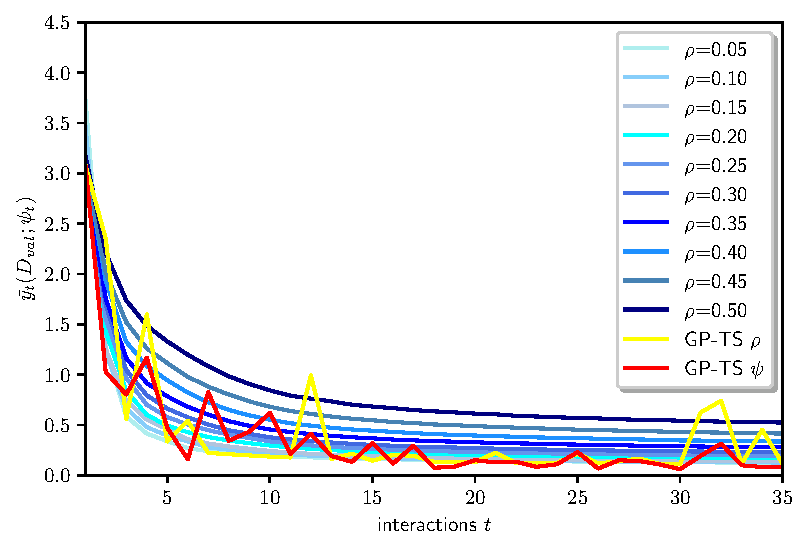
\includegraphics[width=\textwidth]{./figs/wiki_c4_pre_training_loss}
		\vspace*{-4ex}
		\caption{\texttt{wiki-c4}.}
		\label{fig:pretraining_new_wikic4}
	\end{subfigure}
	%
	\begin{subfigure}[c]{0.32\textwidth}
		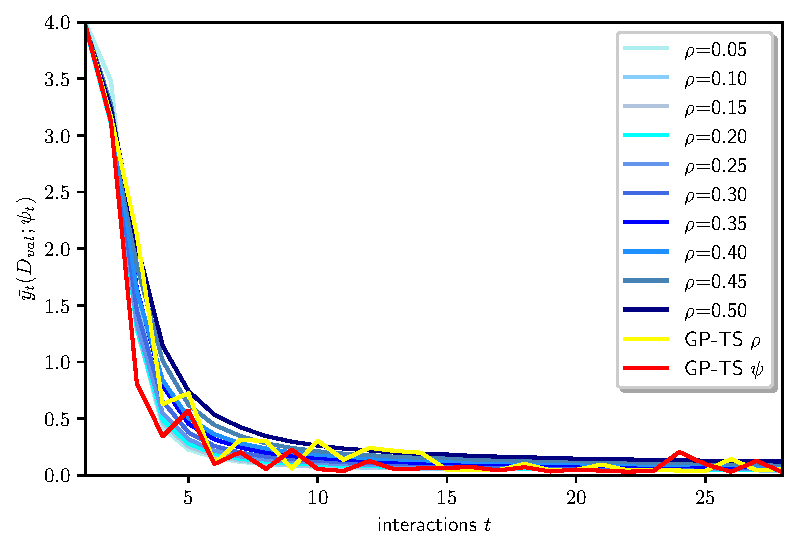
\includegraphics[width=\textwidth]{./figs/medical_new_pre_training_loss}
		\vspace*{-4ex}
		\caption{\texttt{mimic}.}
		\label{fig:pretraining_new_mimic}
	\end{subfigure}
	%
	\begin{subfigure}[c]{0.32\textwidth}
		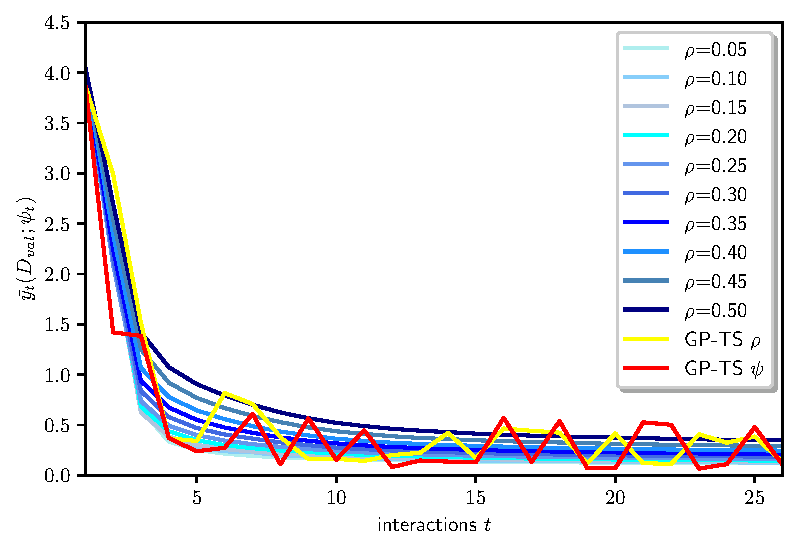
\includegraphics[width=\textwidth]{./figs/ebay_new_pre_training_loss}
		\vspace*{-4ex}
		\caption{\texttt{e-commerce}.}
		\label{fig:pretraining_new_ebay}
	\end{subfigure}
	%
	\vspace*{-1ex}
	\caption{MLM validation loss comparison (lower is better) of grid-search and GP-TS based \textit{from-scratch} pre-trained RoBERTa models, over interactions.
	}
	\label{fig:new_pretraining}
	%\vspace*{-2ex}
\end{figure*}

Results for \textit{continual} pre-training are provided in Figure~\ref{fig:continual_pretraining},
%where we observe that RoBERTa models, when continually pre-trained with GP-TS, achieve the lowest MLM loss in fewer epochs, for both in-domain datasets.
where we observe that GP-TS continually pre-trains the best performing RoBERTa models ---the fastest--- for both in-domain datasets.

\begin{figure}[!h]
	\centering
	%\vspace*{-1ex}
	\begin{subfigure}[c]{0.32\textwidth}
		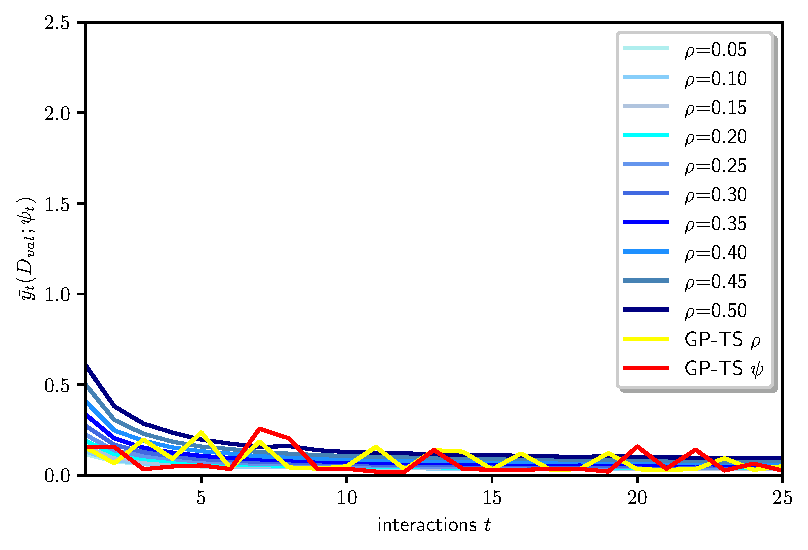
\includegraphics[width=\textwidth]{./figs/medical_robertabase_pre_training_loss}
		\vspace*{-4ex}
		\caption{\texttt{mimic}.}
		\label{fig:continual_pretraining_mimic}
	\end{subfigure}
	%
	\begin{subfigure}[c]{0.32\textwidth}
		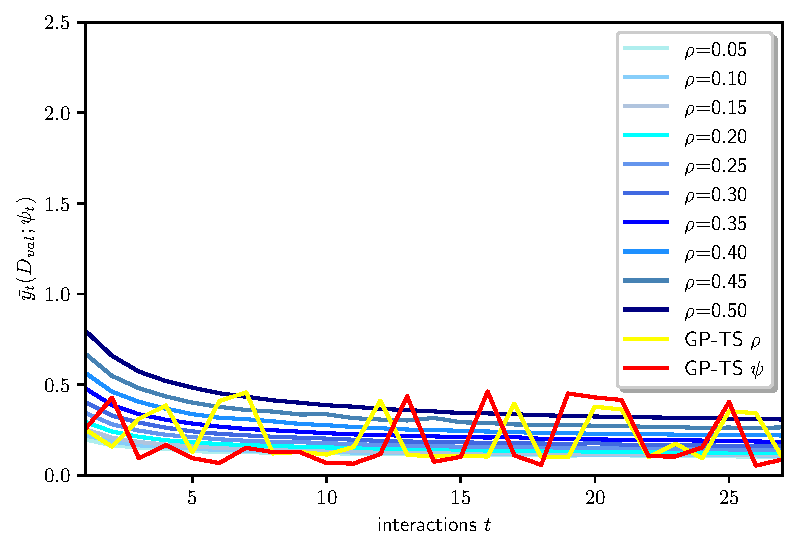
\includegraphics[width=\textwidth]{./figs/ebay_robertabase_pre_training_loss}
		\vspace*{-4ex}
		\caption{\texttt{e-commerce}.}
		\label{fig:continual_pretraining_ebay}
	\end{subfigure}
	\vspace*{-1ex}
	\caption{MLM validation loss comparison (lower is better) of grid-search and GP-TS based \textit{continually} pre-trained RoBERTa models over interactions.
	}
	\label{fig:continual_pretraining}
	%\vspace*{-1ex}
\end{figure}

MLM validation losses for models pre-trained with GP-TS fluctuate across interactions,
depending on the stochastic action (hyperparameter value) selected by the GP-TS agent.

We evaluate the influence of different realizations of GP-TS (with different random seeds) in Table~\ref{tab:medical_MLM_medical_robertabase},
where we observe that GP-TS always pre-trains models with the lowest MLM loss, and in less interactions (indicated within parentheses).
Practitioners are interested in using the model with the lowest validation MLM loss,
which GP-TS consistently finds across all studied datasets and pre-training approaches,
in fewer pre-training interactions.

% Over realizations
% !TEX root = main.tex
\begin{table}[!h]
	\caption{Best MLM loss attained before interactions 20 and 30, when pre-training RoBERTa models continually in the medical domain corpora.}
	\label{tab:medical_MLM_medical_robertabase}
	\vspace*{-1ex}
	\centering
	%\resizebox{\columnwidth}{!}{
		\begin{tabular}{|c|c|c|}
			\hline
		% Main header
		\cellcolor[gray]{0.6} 
			& By interaction 20 \cellcolor[gray]{0.6} 
			& By interaction 30 \cellcolor[gray]{0.6} \\ \cline{1-3}
		\cellcolor[gray]{0.6} 
			& Best MLM loss\cellcolor[gray]{0.8} 
			& Best MLM loss \cellcolor[gray]{0.8} \\ \cline{1-3}
		\multirow{-3}{*}{Model}\cellcolor[gray]{0.6} 
			& (at interaction)\cellcolor[gray]{0.8} 
			& (at interaction)\cellcolor[gray]{0.8} \\ \hline
$\rho$=0.05 	 & 0.04 (18) 	 & 0.037 (28) 	\\ \hline 
$\rho$=0.10 	 & 0.04 (18) 	 & 0.036 (27) 	\\ \hline 
$\rho$=0.15 	 & 0.044 (18) 	 & 0.038 (27) 	\\ \hline 
$\rho$=0.20 	 & 0.048 (18) 	 & 0.042 (28) 	\\ \hline 
$\rho$=0.25 	 & 0.054 (19) 	 & 0.046 (27) 	\\ \hline 
$\rho$=0.30 	 & 0.066 (18) 	 & 0.056 (27) 	\\ \hline 
$\rho$=0.35 	 & 0.076 (19) 	 & 0.064 (29) 	\\ \hline 
$\rho$=0.40 	 & 0.091 (19) 	 & 0.077 (29) 	\\ \hline 
$\rho$=0.45 	 & 0.113 (19) 	 & 0.095 (29) 	\\ \hline 
$\rho$=0.50 	 & 0.134 (19) 	 & 0.112 (27) 	\\ \hline 
\rowcolor[gray]{0.95} 
GP-TS $\rho$ (seed 1) 	 & 0.037 (14) 	 & 0.033 (20) 	\\ \hline 
\rowcolor[gray]{0.95}
GP-TS $\rho$ (seed 2) 	 & 0.036 (19) 	 & 0.033 (28) 	\\ \hline 
\rowcolor[gray]{0.95}
GP-TS $\rho$ (seed 3) 	 & 0.038 (14) 	 & 0.032 (21) 	\\ \hline 
\rowcolor[gray]{0.95}
GP-TS $\rho$ (seed 4) 	 & 0.032 (18) 	 & 0.032 (18) 	\\ \hline 
\rowcolor[gray]{0.95}
GP-TS $\rho$ (seed 5) 	 & 0.038 (13) 	 & 0.032 (20) 	\\ \hline 
GP-TS $\psi$ (seed 1) 	 & 0.027 (8) 	 & 0.019 (21) 	\\ \hline 
GP-TS $\psi$ (seed 2)	 & \textbf{0.02 (15)} 	 & 0.02 (15) 	\\ \hline 
GP-TS $\psi$ (seed 3)	 & \textbf{0.02 (17)} 	 & 0.019 (28) 	\\ \hline 
GP-TS $\psi$ (seed 4)	 & 0.036 (14) 	 & 0.019 (21) 	\\ \hline 
GP-TS $\psi$ (seed 5)	 & \textbf{0.02 (16)} 	 & \textbf{0.018 (28)} 	\\ \hline 
		\end{tabular}
	%}
\vspace*{-1ex}
\end{table}

%
GP-TS not only circumvents the need for costly grid searches, but enables improved performance:
it attains reduced MLM loss at earlier interactions than grid-search baselines.
Recall how GP-TS $\psi$ outperforms all the alternatives in Table~\ref{tab:medical_MLM_medical_robertabase},
as it pre-trains models with the lowest MLM, the fastest
---even when no good initial guesses for the MLM hyperparameters $\psi=\left(\rho, \gamma, \lambda\right)$ are available.

In summary, the benefits of interactive GP-TS pre-training do not pertain to the attained MLM values only,
but to an accelerated, efficient procedure.
We emphasize the computational efficiency of GP-TS:
it adds little to no overhead ---details on the computational cost of GP-TS are provided in Appendix~\ref{asec:computational_overhead}---
while providing clear benefits for language model pre-training.
It attains best MLM pre-training performance in less interactions,
avoiding computationally expensive hyperparameter search.

To the best of our knowledge, these experiments provide novel evidence that,
instead of MLM pre-training with fixed masking hyperparameters,
sequentially deciding which masking values to use is beneficial.
Namely, GP-TS finds \textit{sequences} of dynamic masking hyperparameters
(when optimizing over $\rho$ or a three-dimensional hyperparameter space $\psi\in\Psi$)
that minimize MLM loss across datasets, when pre-training from-scratch and continually.


%Finally, we recall that by inspecting the GP posterior of the GP-TS agent (see Figures provided in Appendix~\ref{asec:gpts_posterior}), we can learn about which hyperparameters have more influence on the pre-training procedure; \ie which hyperparameter values help reduce validation loss.
%GP-TS favours dynamic masking probability values in $\rho=(0.05,1.20)$ when pre-training with \texttt{wiki-c4} data, while for the in-domain datasets, the posterior is much flatter.
%We hypothesize that such a difference is related to the different linguistic nature of the pre-training corpora:
%\texttt{wiki-c4} contains redacted, long sentences; while \texttt{eBay} and \texttt{mimic} data are sequences of succinct, not necessarily fully redacted, descriptions.
%Nevertheless, no matter which dynamic hyperparameters are favored, GP-TS achieves successful pre-training in all the studied cases:
%\ie it avoids costly hyperparameter grid-search, yet attains best MLM validation loss in less epochs.

\subsection{GP-TS pre-trained RoBERTa models for downstream fine-tuned tasks}
\label{ssec:downstream}

We scrutinize how performant in-domain GP-TS pre-trained RoBERTa models are,
when compared to grid-search based models,
after in-domain per-task fine-tuning.
We note that the downstream, fine-tuned performance of RoBERTa models pre-trained from-scratch with in-domain data is, as expected, lower than if continually pre-trained.

The fine-tuned accuracy of continually pre-trained models
of Figure~\ref{fig:continual_pretraining} are presented in Table~\ref{tab:ebay_tasks_robertabase}:
we showcase best (per-task) test-set accuracy for each fine-tuned model,
and at which pre-training interaction was such value attained.
Results are computed on each per-task test-set,
\ie a subset of each task's dataset (see details in Table~\ref{tab:finetuning_dataset_details})
that has not been used for fine-tuning nor hyperparameter optimization.

% continual results only
% !TEX root = ../main.tex
\begin{table}[!h]
	\caption{Best fine-tuned, downstream task test-set accuracy (higher is better) for continually pre-trained RoBERTa models.
		The first row corresponds to the fine-tuned performance of the RoBERTa model from which continual pre-training is started.}
	\label{tab:ebay_tasks_robertabase}
	%\vspace*{-1ex}
	\centering
	%\resizebox{\columnwidth}{!}{
		\begin{tabular}{|c|c|c|c|c|}
			\hline
			% Main header
			\cellcolor[gray]{0.6} 
			& e-commerce \cellcolor[gray]{0.6} 
			& e-commerce \cellcolor[gray]{0.6} 
			& e-commerce \cellcolor[gray]{0.6}
			& medical \cellcolor[gray]{0.6} \\ \cline{1-5}
			\cellcolor[gray]{0.6} 
			& title classification \cellcolor[gray]{0.6} 
			& title similarity \cellcolor[gray]{0.6} 
			& title quality \cellcolor[gray]{0.6}
			& MLI \cellcolor[gray]{0.6} \\ \cline{1-5}
			\cellcolor[gray]{0.6} 
			& Accuracy\cellcolor[gray]{0.8} 
			& Accuracy\cellcolor[gray]{0.8} 
			& Accuracy\cellcolor[gray]{0.8} 
			& Accuracy\cellcolor[gray]{0.8} \\ \cline{1-4}
			\multirow{-4}{*}{Model}\cellcolor[gray]{0.6} 
			& (at interaction)\cellcolor[gray]{0.8} 
			& (at interaction)\cellcolor[gray]{0.8} 
			& (at interaction)\cellcolor[gray]{0.8} 
			& (at interaction)\cellcolor[gray]{0.8} \\ \hline
RoBERTa base 	 & 97.2 \;\;(0) 	 & 97.2 \;\;(0) 	 & 75.1 \;\;(0) 	 & 67.5 \;\;(0) 	\\ \hline 
$\rho$=0.05 	 & 97.8 (26) 	 & 97.8 (26) 	 & 77.6 (15) 	 & 72.9 \;\;(3) 	\\ \hline 
$\rho$=0.10 	 & 97.9 (27) 	 & 97.9 (27) 	 & 77.7 (15) 	 & 71.9 \;\;(9) 	\\ \hline 
$\rho$=0.15 	 & 97.8 (13) 	 & 97.8 (13) 	 & 77.7 (18) 	 & 72.5 (13) 	\\ \hline 
$\rho$=0.20 	 & 97.8 \;\;(8)	 & 97.8 \;\;(8) 	& 77.4 (10) 	 & 73.3 (14) 	\\ \hline 
$\rho$=0.25 	 & 97.9 (17) 	& 97.9 (17) 	 & 77.7 \;\;(6)	 & 72.9 (12) 	\\ \hline 
$\rho$=0.30 	 & 97.9 (19)	& 97.9 (19) 	& 77.8 \;\;(7)	 & \textbf{73.2 \;\;(7)} 	\\ \hline 
$\rho$=0.35 	 & 97.9 \;\;(9)	 & 97.9 \;\;(9) 	& 77.8 (18) 	 & 72.8 \;\;(7) 	\\ \hline 
$\rho$=0.40 	 & 97.8 \;\;(9)	 & 97.8 \;\;(9) 	& 78.2 (24) 	 & 72.6 \;\;(9) 	\\ \hline 
$\rho$=0.45 	 & 97.8 (11) 	 & 97.8 (11) 	 & \textbf{78.3 (16)} 	 & 72.9 \;\;(7) 	\\ \hline 
$\rho$=0.50 	 & 97.9 \;\;(8)	 & 97.9 \;\;(8) 	& 77.9 \;\;(7)	 & 72.6 \;\;(9) 	\\ \hline 
GP-TS $\rho$ 	 & 97.9 (13) 	 & 97.9 (13) 	 & 77.5 (17) 	 & 72.6 \;\;(9) 	\\ \hline 
GP-TS $\psi$ 	 & \textbf{98.0 (10)} 	 & \textbf{98.0 (10)} 	 & 77.8 (20) 	 & 72.3 \;\;(6) 	\\ \hline 
		\end{tabular}
	%}
%\vspace*{-1ex}
\end{table}

These results exhibit how GP-TS pre-trains performant language models ---with top accuracy---
often at earlier interactions than when pre-training with static hyperparameters:
\eg the continually pre-trained GP-TS $\psi$ model
(see last row of Table~\ref{tab:ebay_tasks_robertabase})
provides best downstream accuracy for two e-commerce tasks and competitive accuracy in others,
in just a few pre-training interactions.

\clearpage
This efficiency is of practical importance,
due to the significant resource savings it affords.
A pre-training hyperparameter grid-search
does not provide significant downstream performance improvements,
yet it demands high computational resources
---the computational complexity of a grid-search over hyperparameters $\psi=\left(\rho, \gamma, \lambda\right)$ with $n$ candidates per hyperparameter is $\mathcal{O}(3^n)$.
%
On the contrary, by letting GP-TS pre-train TLMs,
best pre-training MLM performance is achieved,
with well-performing fine-tuned model accuracy across downstreams tasks,
in fewer pre-training interactions.

%Presented evidence demonstrates that GP-TS enables fast and superior pre-training of language models:
%not only is GP-TS able to accelerate and improve MLM pre-training,
%but it results in robust TLMs that can be quickly fine-tuned to downstream tasks with excellent accuracy.
